\documentclass[journal, a4paper]{IEEEtran}
\usepackage[T1]{fontenc}       % Encodage le plus étendu
\usepackage[utf8]{inputenc}    % Source Unicode en UTF-8

\usepackage[cyr]{aeguill}
\usepackage[francais]{babel} % Pour la redaction du document en francais


% some very useful LaTeX packages include:

%\usepackage{cite}      % Written by Donald Arseneau
                        % V1.6 and later of IEEEtran pre-defines the format
                        % of the cite.sty package \cite{} output to follow
                        % that of IEEE. Loading the cite package will
                        % result in citation numbers being automatically
                        % sorted and properly "ranged". i.e.,
                        % [1], [9], [2], [7], [5], [6]
                        % (without using cite.sty)
                        % will become:
                        % [1], [2], [5]--[7], [9] (using cite.sty)
                        % cite.sty's \cite will automatically add leading
                        % space, if needed. Use cite.sty's noadjust option
                        % (cite.sty V3.8 and later) if you want to turn this
                        % off. cite.sty is already installed on most LaTeX
                        % systems. The latest version can be obtained at:
                        % http://www.ctan.org/tex-archive/macros/latex/contrib/supported/cite/

\usepackage{graphicx}   % Written by David Carlisle and Sebastian Rahtz
                        % Required if you want graphics, photos, etc.
                        % graphicx.sty is already installed on most LaTeX
                        % systems. The latest version and documentation can
                        % be obtained at:
                        % http://www.ctan.org/tex-archive/macros/latex/required/graphics/
                        % Another good source of documentation is "Using
                        % Imported Graphics in LaTeX2e" by Keith Reckdahl
                        % which can be found as esplatex.ps and epslatex.pdf
                        % at: http://www.ctan.org/tex-archive/info/

%\usepackage{psfrag}    % Written by Craig Barratt, Michael C. Grant,
                        % and David Carlisle
                        % This package allows you to substitute LaTeX
                        % commands for text in imported EPS graphic files.
                        % In this way, LaTeX symbols can be placed into
                        % graphics that have been generated by other
                        % applications. You must use latex->dvips->ps2pdf
                        % workflow (not direct pdf output from pdflatex) if
                        % you wish to use this capability because it works
                        % via some PostScript tricks. Alternatively, the
                        % graphics could be processed as separate files via
                        % psfrag and dvips, then converted to PDF for
                        % inclusion in the main file which uses pdflatex.
                        % Docs are in "The PSfrag System" by Michael C. Grant
                        % and David Carlisle. There is also some information
                        % about using psfrag in "Using Imported Graphics in
                        % LaTeX2e" by Keith Reckdahl which documents the
                        % graphicx package (see above). The psfrag package
                        % and documentation can be obtained at:
                        % http://www.ctan.org/tex-archive/macros/latex/contrib/supported/psfrag/

%\usepackage{subfigure} % Written by Steven Douglas Cochran
                        % This package makes it easy to put subfigures
                        % in your figures. i.e., "figure 1a and 1b"
                        % Docs are in "Using Imported Graphics in LaTeX2e"
                        % by Keith Reckdahl which also documents the graphicx
                        % package (see above). subfigure.sty is already
                        % installed on most LaTeX systems. The latest version
                        % and documentation can be obtained at:
                        % http://www.ctan.org/tex-archive/macros/latex/contrib/supported/subfigure/

\usepackage{url}        % Written by Donald Arseneau
                        % Provides better support for handling and breaking
                        % URLs. url.sty is already installed on most LaTeX
                        % systems. The latest version can be obtained at:
                        % http://www.ctan.org/tex-archive/macros/latex/contrib/other/misc/
                        % Read the url.sty source comments for usage information.

%\usepackage{stfloats}  % Written by Sigitas Tolusis
                        % Gives LaTeX2e the ability to do double column
                        % floats at the bottom of the page as well as the top.
                        % (e.g., "\begin{figure*}[!b]" is not normally
                        % possible in LaTeX2e). This is an invasive package
                        % which rewrites many portions of the LaTeX2e output
                        % routines. It may not work with other packages that
                        % modify the LaTeX2e output routine and/or with other
                        % versions of LaTeX. The latest version and
                        % documentation can be obtained at:
                        % http://www.ctan.org/tex-archive/macros/latex/contrib/supported/sttools/
                        % Documentation is contained in the stfloats.sty
                        % comments as well as in the presfull.pdf file.
                        % Do not use the stfloats baselinefloat ability as
                        % IEEE does not allow \baselineskip to stretch.
                        % Authors submitting work to the IEEE should note
                        % that IEEE rarely uses double column equations and
                        % that authors should try to avoid such use.
                        % Do not be tempted to use the cuted.sty or
                        % midfloat.sty package (by the same author) as IEEE
                        % does not format its papers in such ways.

\usepackage{amsmath}    % From the American Mathematical Society
                        % A popular package that provides many helpful commands
                        % for dealing with mathematics. Note that the AMSmath
                        % package sets \interdisplaylinepenalty to 10000 thus
                        % preventing page breaks from occurring within multiline
                        % equations. Use:
%\interdisplaylinepenalty=2500
                        % after loading amsmath to restore such page breaks
                        % as IEEEtran.cls normally does. amsmath.sty is already
                        % installed on most LaTeX systems. The latest version
                        % and documentation can be obtained at:
                        % http://www.ctan.org/tex-archive/macros/latex/required/amslatex/math/

\usepackage{lipsum} % Dummy text


% Other popular packages for formatting tables and equations include:

%\usepackage{array}
% Frank Mittelbach's and David Carlisle's array.sty which improves the
% LaTeX2e array and tabular environments to provide better appearances and
% additional user controls. array.sty is already installed on most systems.
% The latest version and documentation can be obtained at:
% http://www.ctan.org/tex-archive/macros/latex/required/tools/

% V1.6 of IEEEtran contains the IEEEeqnarray family of commands that can
% be used to generate multiline equations as well as matrices, tables, etc.

% Also of notable interest:
% Scott Pakin's eqparbox package for creating (automatically sized) equal
% width boxes. Available:
% http://www.ctan.org/tex-archive/macros/latex/contrib/supported/eqparbox/

% *** Do not adjust lengths that control margins, column widths, etc. ***
% *** Do not use packages that alter fonts (such as pslatex).         ***
% There should be no need to do such things with IEEEtran.cls V1.6 and later.


% En-tête et pied de page
%\usepackage{lastpage}
%\usepackage{fancyhdr}
%\pagestyle{fancy}
%\renewcommand{\sectionmark}[1]{\markright{#1}}
%\fancyhead{}
%%\fancyhead[RO,LE]{\slshape\footnotesize\nouppercase{\rightmark}}
%\fancyhead[LO,RE]{\thetitle}
%\fancyfoot{}
%%\fancyfoot[LO,RE]{\footnotesize\texttt{\thefilename}\\ \textit{\now}}
%%\fancyfoot[C]{-~\thepage~/~\pageref{LastPage}~-}
%\fancyfoot[RO,LE]{\raisebox{-2mm}{\includegraphics{structure/barrette-original}}}
%%
%\fancypagestyle{plain}{ %  Première page ----------------------
%  \fancyhead{}
%  \renewcommand{\headrulewidth}{0pt}
%  \fancyheadoffset[R]{15mm}
%  \fancyhead[L]{
%    \raisebox{-7mm}{
%      \parbox{\textwidth}{
%        \includegraphics{structure/barrette-original} \\ \\
%        \fontsize{8pt}{10pt}\selectfont
%        \sffamily\color{Pantone287}
%        FACULTÉ DES SCIENCES       \\
%        DÉPARTEMENT D'INFORMATIQUE   
%      }
%    }
%  }
%  \fancyhead[R]{
%    \raisebox{-10mm}[0pt][0pt]{\includegraphics[width=120mm]{structure/ULB-ligne-gauche}}
%  }
%  \fancyfoot{}
%  %\fancyfoot[L]{\raisebox{0mm}{}\color{Pantone287}\footnotesize\texttt{\thefilename}\\ \textit{\now}}
%  %\fancyfoot[C]{-~\thepage~/~\pageref{LastPage}~-}
%  \fancyfoot[R]{
%    \raisebox{-12pt}{\includegraphics[height=\footskip]{structure/sceau-mini-b-quadri}}
%  }
%} % Fin de première page
% ---------------------------------------------------------------------------


\usepackage{listings}

% Your document starts here!
\begin{document}

% Define document title and author
	\title{L'algorithme génétique pour apprendre à une IA à marcher.}
	\author{Robin-Gilles Becker
	\thanks{Superviseur: xxx}}
	\markboth{INFO-F308}{}
	\maketitle

% Write abstract here
\begin{abstract}

	Cet article présente l'analyse de l'utilisation de l'algorithme génétique dans le contexte d'une intelligence artificielle prenant la forme d'une créature quadrupède et devant apprendre à marcher le plus loin possible sur un sol plat. La méthode d'apprentissage a été implémentée avec Pygad \cite{PyGad} et, pour la simulation en 3D de notre créature, nous utilisons le moteur physique PyChrono \cite{PyChrono}. Nous concluons que trouver les valeurs optimales des paramètres de reproduction, mutation et sélection avec la fitness function, ainsi que des caractéristiques physiques de l'environnement de la simulation est essentiel pour obtenir de bons résultats. Mais nous en retirons surtout l'importance vitale de l'optimisation des performances du procédé, sans quoi il est impossible d'atteindre des résultats satisfaisants.


%	Le résumé (80-100 mots) est conçu pour donner au lecteur une vue générale du contenu de l'article. 







 
\end{abstract}

% Each section begins with a \section{title} command
\section{Introduction}

\PARstart{C}{es} dernières années, le développement des robots capables de marcher a suscité une intérêt croissant dans le domaine de la robotique, puisqu'ils sont plus adaptés pour se déplacer sur des terrains difficiles que ceux à roues. Parvenir à des comportements de marche stables et naturels chez les robots représente un défi complexe nécessitant des méthodes d'apprentissage efficaces.

A cette échelle de complexité, il est évident que trouver le meilleur algorithme, la méthode la plus efficace, est primordial dans l'obtention de résultats de qualité. Ainsi, nous avons choisi d'étudier l'algorithme génétique, une approche inspirée de l'évolution biologique, où une population d'individus est soumise à des processus de sélection, de reproduction et de mutation pour générer des solutions optimisées.

La réalisation d'une telle tâche présente d'importants défis, comme le maintient de l'équilibre, la coordination,... Pour faciliter l'apprentissage de notre créature, nous avons choisi de créer un quadrupède, qui aura plus facile à se tenir en équilibre qu'un bipède.
Cependant, le défi le plus important est celui de l'optimisation. Les algorithmes nécessitant d'être exécuter des milliers de fois durant le procédé permettant à l'IA de converger vers son objectif, chaque instant compte. La formule de la fonction heuristique, le nombre d'individus par génération, le nombre d'individus gardés pour reproduction, le nombre de parent gardés à la génération suivante, la structure du génome des créatures, les données physiques du monde de la simulation,... Tous ces paramètres se doivent d'être réfléchis et choisis avec minutie pour un résultat optimal. C'est dans cette optique que nous utilisons PyGad \cite{PyGad}, une librairie python créée spécifiquement pour mettre en place des algorithmes génétiques et permettant de modifier les paramètres sus-mentionnés.

L'objectif de cet article est d'expliquer l'algorithme mise en place, les problèmes rencontrés et les résultats. Après avoir exploré l'état de l'art, nous établirons nos choix de conception quant aux 2 méthodes d'apprentissage et expliquerons la façon dont nous avons procédé. Nous discuterons des problèmes rencontrés et finirons par comparer les résultats obtenus avant de discuter des possibles améliorations qui pourraient être rajoutées.


	% \PARstart{}{} creates a tall first letter for this first paragraph
%	\PARstart{C}{ette} section donne une introduction générale du problème scientifique abordé et décrit la structure de l'article. Des questions souvent abordées ici sont :
%	\begin{itemize}
%	\item Quelles sont les applications du problème abordées ?
%	\item Pourquoi la résolution du problème est importante ?
%	\end{itemize}	  

\section{État de l'art}

Dans notre projet, nous utilisons un algorithme génétique classique. Le génome de l'algorithme est modélisé par une liste de valeurs discrètes représentant les forces à appliquer à chaque unité de temps (timestep) de la simulation, et ce pour chaque membre de la créature rattaché à un joint. Les données et paramètres sont envoyés à PyGad qui se charge d'exécuter l'algorithme. Notre fitness function vise à récompenser la distance effectuée et la vitesse de marche, tandis que les chûtes sont pénalisées.

Dans le reste de la littérature, diverses approches ont été explorées pour résoudre la problématique de l'optimisation de l'apprentissage de la marche, notamment l'utilisation de techniques avancées pour améliorer l'algorithme employé. Dans cette section, nous présenterons un aperçu de l'état de l'art de l'algorithme génétique pour apprendre aux intelligences artificielles à marcher.

% --

Une des approches \cite{1-evol} met en place une approche originale pour enseigner à un robot à marcher en utilisant un algorithme génétique. Cette approche adopte une perspective différente en se concentrant sur le mouvement du corps plutôt que sur les jambes. La trajectoire du corps est représentée par un modèle d'accélération qui maintient la direction de déplacement souhaitée. Le comportement de chaque jambe dépend de la position du pied, qu'il soit en l'air ou au sol. Lorsque le pied est au sol, la jambe se déplace par rapport au corps pour satisfaire la contrainte cinématique du mouvement du corps sans glissement. Lorsque le pied est en l'air, la jambe se déplace vers un point cible spécifié où elle sera posée.

Les paramètres de mouvement sont définis pour permettre à chaque pied de quitter le sol tout en avançant, sans spécifier le chemin exact à suivre. Les individus sont évalués en fonction de leur vitesse de déplacement vers l'avant, mesurée par la distance parcourue pendant une période de temps donnée.

Pour maintenir la diversité de la population et éviter la stagnation dans des optimums locaux, des populations qui se chevauchent partiellement sont utilisées. De plus, un mécanisme de radiation est utilisé pour augmenter le taux de mutation dans les zones où de nombreux individus sont regroupés, favorisant ainsi la dispersion des solutions dans l'espace de recherche. C'est un procédé de mutation plus avancé que celui qu'on trouve en général dans les algorithmes génétiques tels que celui de notre projet. Les paramètres des opérateurs de reproduction et de mutation sont ajustés au fil des phases de l'algorithme pour passer d'une exploration globale à une exploration plus détaillée des régions environnantes des solutions prometteuses.

Des précautions supplémentaires ont été prises pour éviter que des résultats anormalement élevés ne faussent l'évaluation des individus, notamment en effectuant plusieurs évaluations successives pour les individus les plus prometteurs.

% --

Un article sur le déplacement de robots à huit pattes utilise un algorithme génétique avec une notion de phase et de point de référence \cite{2-eigth} pour contrôler le mouvement de chaque patte, où une phase de 0 signifie que la patte est en phase avec le point de référence, tandis qu'une phase d'une demi signifie qu'elle est déphasée de 180 degrés.

La fitness de chaque individu est évaluée en utilisant la marge de stabilité minimale, mesurée pendant une simulation de marche de 30 secondes. Cette marge de stabilité minimale est ensuite mise au carré pour augmenter les différences entre les individus et favoriser l'évolution de démarches présentant une stabilité élevée.

La notion de phase permet de contrôler finement le mouvement de chaque patte, tandis que l'évaluation de la fitness favorise l'évolution de démarches stables.

% --

Il est aussi possible d'utiliser l'algorithme génétique pour optimiser la morphologie de créatures virtuelles en faisant évoluer leur génome \cite{siggraph}, qui représente leur corps sous la forme de graphes dirigés composés de noeuds et de connexions. Tout comme les créatures de notre projet, leur corps se compose de parties rigides articulées en trois dimensions, permettant une simulation physique réaliste. La créature utilise un réseaux neuronal qui traite les valeurs de capteurs sensoriels et génère des valeurs d'effecteurs de sortie, lesquelles sont appliquées sous forme de forces aux articulations du corps de la créature. Les descriptions génotypiques des cerveaux virtuels et leurs phénotypes correspondants sont aussi tous deux représentés sous forme de graphes dirigés. L'algorithme génétique évalue la fitness des créatures dans le monde virtuel simulé et la survie et la reproduction des créatures en dépendent : les individus les plus performants donnant naissance à une descendance grâce à des opérations de reproduction et de mutation. La particularité est l'utilisation de plusieurs types de reproduction choisis au hasard. Ainsi, non seulement le comportement de la créature, mais aussi son corps, évolue en fonction de la situation.

Cet algorithme génétique a été fait pour s'exécuter en parallèle sur des super-ordinateurs, permettant une croissance efficace avec une augmentation du nombre de processeurs.

Dans notre projet, nous ne modifions pas le corps de la créature une fois créé, mais nous utilisons aussi un génome composé de forces à appliquer aux joints.

% --

%Du côté du reinforcement learning (RL), une équipe a modélisé le problème comme un Processus de Décision Markovien (MDP) à espace d'états continu \cite{4-reinf}, où l'objectif est d'apprendre une politique qui maximise les récompenses totales au cours d'un épisode. Deux algorithmes de RL off policy ont été considérés : Soft Actor Critic (SAC) et Twin Delayed Deep Deterministic Policy Gradients (TD3). Le premier maximise l'entropie de la politique en plus de la récompense attendue, ce qui encourage l'exploration de l'état de l'agent. Le second utilise deux Q-functions, une mise à jour différée de la policy et du noise sur l'action cible pour améliorer les performances. 

%Dans ce contexte, les états du robot comprennent les informations sur son orientation et ses articulations, tandis que les actions correspondent à des contrôles de position pour les articulations. Une fonction de récompense a été conçue pour encourager le robot à marcher le plus loin possible avec une consommation d'énergie minimale. Différents modèles de mouvement ont été explorés, notamment une trajectoire en forme de sinus, une trajectoire en forme de rose et une trajectoire en forme de triangle.

%Les auteurs ont également utilisé plusieurs optimiseurs pour trouver les paramètres optimaux lors du processus d'entraînement, tels que Covariance Matrix Adaptation Evolution Strategy (CMAES), Test-Based Population Size Adaptation (TBPSA) et Bayesian Optimisation (BO).

% ---

%Une autre approche est celle du Continuous-Action Q-Learning (CAQ) \cite{5-QL} pour étendre l'action space discret à un action space continus. L'algorithme utilise une distribution gaussienne pour enregistrer la récompense future maximale attendue et l'action associée. L'idée principale est d'adapter le RL classique en utilisant des actions continues au lieu d'actions discrètes, ce qui rend les actions plus habiles et améliore les résultats. La fonction de récompense est conçue en se basant sur la position du Centre de Pression du robot (ZMP), offrant des récompenses positives lorsque le robot se déplace vers l'avant avec un bon équilibre, et des récompenses négatives lorsqu'il est instable ou tombe. L'algorithme ajuste la moyenne et la variance de la distribution gaussienne afin d'augmenter la probabilité de générer une sortie réelle optimale pour chaque état. Cette approche permet de bien contrôler les mouvements du robot bipède et d'optimiser son apprentissage de la marche.

% --

%Dans une autre variante du RL \cite{9-deep}, l'accent est mis sur le compromis entre l'exploitation maximale des récompenses et l'exploration de l'incertitude, qui est directement influencé par l'échelle de la fonction de récompense. Contrairement au RL conventionnel, où la policy optimale est indépendante de l'échelle de la reward function, dans le RL à entropie maximale, le facteur d'échelle doit être ajusté pour chaque environnement.

%L'objectif est d'optimiser l'entropie maximale de la policy tout en permettant une variation de l'entropie à différents états. Pour résoudre ce problème, une relaxation lagrangienne est utilisée, conduisant à l'objectif d'entropie maximale par rapport à la policy. Cette approche est optimisée à l'aide de la méthode du Dual Gradient (DG).

%La policy est paramétrée à l'aide d'une distribution gaussienne, et ses paramètres sont appris à l'aide de la Stochastic Gradient Descent (SGD) et l'algorithme proposé alterne entre une phase de collecte de données et une phase d'optimisation.

% --

%Pour aller plus loin dans le RL, une autre étude se repose sur la définition d'un state space basé sur les mesures des capteurs disponibles sur le robot ainsi qu'un réseau neuronnal \cite{8-deep}. Le space state correspond aux angles de rotation de référence des moteurs, permettant un contrôle continu.

%Pour guider l'apprentissage, des récompenses constantes sont attribuées au robot pour rester équilibré, en vie et maintenant une vitesse de déplacement positive dans la direction souhaitée à chaque instant.

%L'apprentissage est réalisé à l'aide de réseaux neuronaux et de l'algorithme PPO.

% --

%Un autre amélioration \cite{7-FSM} met en place un contrôleur basé sur une Finite State Machine (FSM) et un réseaux neuronal. La FSM comprend 4 états représentant un cycle de locomotion, où chaque état définit les angles cibles des articulations pour le contrôle PD. Le robot effectue des mouvements de balancement de la jambe pendant les états de balancement vers le haut, puis abaisse la jambe pendant les états de balancement vers le bas pour entrer en contact avec le sol.

%Le contrôleur apprend également à régler la durée des états de balancement vers le haut et les autres articulations, telles que les genoux, les chevilles et les articulations du haut du corps.

%Le contrôle de la marche est réalisé en exploitant la nature discrète de la FSM, où les transitions d'état et les mises à jour des angles cibles se produisent principalement en fonction des pas. Ici, l'apprentissage se fait par RL avec l'algorithme PPO doublé d'un réseau neuronal représentant la politique de contrôle qui optimise les paramètres de la marche, tels que les angles des articulations.

%L'article met également en évidence l'importance de la sélection judicieuse des récompenses et des termes de pénalité pour guider l'apprentissage. Les récompenses et les pénalités sont définies en fonction de la déviation par rapport aux paramètres de marche souhaités, du maintien de la posture du haut du corps, de la direction vers l'avant et de l'effort des articulations.

%Cette approche offre une méthode prometteuse pour l'apprentissage de la marche chez les robots en utilisant un contrôleur basé sur un FSM et l'algorithme PPO. Les expérimentations montrent que cette approche permet d'obtenir des mouvements de marche plus naturels et stables.

% --

Non seulement l'algorithme génétique peut être combiné avec un réseau neuronal, mais aussi avec d'autres algorithmes, comme le reinforcement learning \cite{6-control}. L'objectif de cette approche est d'améliorer la vitesse et la stabilité de la marche avec le concept de Zero Moment Point (ZMP) pour évaluer la marche, où le ZMP est défini comme le point sur le sol où la force de réaction du sol s'annule avec la gravité et l'inertie. L'apprentissage par RL est formulé comme un Processus de Décision Markovien (MDP) et optimisé à l'aide de l'algorithme Proximal Policy Optimization (PPO). L'algorithme génétique est utilisé quant à lui pour ajuster les paramètres du modèle de marche en optimisant diverses variables telles que la longueur et la largeur des pas, l'angle des pas, la hauteur de la jambe en mouvement, etc. Encore une fois, la fitness function favorise la marche stable et rapide vers l'avant, tandis que les déviations et les chutes sont pénalisées. Nous essayons de favoriser et pénaliser les mêmes paramètres dans notre fitness function.

% --

Une autre approche basée sur un algorithme génétique pour trouver une locomotion bipède stable utilise 7 constantes liées aux articulations des jambes \cite{3-arms}. Ils utilisent des fonctions périodiques pour générer les trajectoires angulaires des articulations de la hanche et du genou, en maintenant les pieds parallèles au sol en tout temps. De plus, les articulations équivalentes des jambes suivent les mêmes trajectoires avec un déphasage de $π$. Les paramètres de marche sont évalués en utilisant une équation prenant en compte la performance de la marche avec pénalités en cas d'événements indésirables.

Pour surmonter les problèmes de chute du robot lors des premiers pas et d'évaluation erronée des paramètres de marche, les auteurs ont implémenté deux heuristiques. Tout d'abord, le mouvement a été initié avec des amplitudes linéairement croissantes pendant les premiers pas. Ensuite, au lieu d'utiliser une seule exécution pour évaluer un ensemble de paramètres de marche, la moyenne de trois marches a été prise en compte.
\\ \\
Ainsi, il est intéressant de remarquer qu'il existe plusieurs autres approches complètement différentes aux procédés de reproduction, évaluation de fitness, mutation, conception des créatures, génome et backend.



%	Cette section permet de décrire l'état de l'art concernant la question abordée (c-à-d les meilleures solutions disponibles à présent) et de positionner votre travail par rapport à cet état de l'art.
%	Les différents articles que vous avez lus et utilisés doivent être correctement référencés (Exemple: \cite{small},\cite{big}).
%	Les informations bibliographiques doivent être encodées dans le fichier \texttt{References.bib} avec la syntaxe indiquée par les exemples.
%	Articles publiés sur une revue scientifique / dans les conference proceedings, ainsi que des livres, sont des exemples de bonnes références.
%	Par contre, la citation de sources web doit être limitée le plus possible (permis dans le cas de la documentation d'outils informatiques).

% Main Part
\section{Méthodologie}\label{sec:met}

\subsection{Génome}
  
Le génome de nos créatures est la suite déterministe de valeurs que l'algorithme génétique va chercher à optimiser. Nous avons choisi de représenter ce génome par une array de forces pour chaque joint, qui décrivent les forces qui vont être appliquées au membre rattaché à ce joint à chaque instant (timestep). Ces arrays sont ensuite fusionnées en une seule, qui constitue le génome.
Notons aussi que les valeurs des forces sont limitées à des mouvements faisables par les membres de la créature. Ainsi, nous n'aurons pas de pattes qui feront des tours complets. La façon dont ces valeurs sont limitées sera abordée dans la section consacrée à l'utilisation de PyGad.

\begin{figure}[!htb]
  \centering
  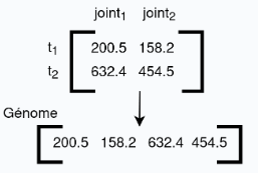
\includegraphics[width=0.25\textwidth]{RapportScientifiqueTemplate/2023-05-23 docs.google.com 9f7a5d7d74de.png}
  \caption{Exemple réduit de la construction d'un génome avec 2 joints et pour 2 timesteps}
  \label{fig:example}
\end{figure}

Le génome est déterministe, ce qui signifie qu'il peut être sauvé dans un fichier et que jouer une simulation en attribuant ce génome à la créature donnera toujours les mêmes mouvements. Cette particularité sera très importante pour la suite, car nous pouvons alors réutiliser les meilleurs résultats d'entraînements passés pour commencer de nouveaux entraînements à partir de ceux là. En effet, lors de la première génération, au début de l'algorithme, les génomes de chaque individus sont générés aléatoirement. A partir de là, l'algorithme est censé les faire converger vers des valeurs produisant des résultats positifs. Cependant, recommencer de zéro à chaque fois, à partir de génomes aléatoires, devient rapidement une perte de temps une fois que nous possédons déjà des génomes ayant de bons résultats. Bien que recommencer du début permet d'explorer un champs de possibilités plus étendus, il vient un moment où le progrès se fera principalement à partir de solutions déjà prometteuses. D'où l'importance d'avoir des génomes qui peuvent être réutilisés.


\subsection{Fitness Function}

Un élément clé d'un bon apprentissage avec algorithme génétique est la définition de la fitness function. C'est la formule qui va évaluer l'aptitude de chaque individu et leur attribuer plus ou moins de points selon les critères choisis.
Notre fitness function est la suivante. Elle représente la valeur de la fitness pour un individu à un instant $i$.

\begin{equation} 
\text{{Fitness}} = \text{{ alive\_bonus }} + ((\text{{ H}}_\text{i-1 }-\text{{ H}}_\text{i }) * 0.1 )
\end{equation}
\[
  + \text{{ D}}_\text{i-1} / 2 + \text{{ D}}_\text{i-1} / time + \text{{ forces }}
\]

La première pénalité est l'une des plus essentielles. \\
La composante \text{{alive\_bonus}} encourage la continuité du mouvement en attribuant un bonus lorsque le tronc de l'agent ne touche pas le sol. Dans cette situation, la valeur de \text{{alive\_bonus}} est augmentée de 0.5 à chaque timestep, tandis qu'une pénalité de 0.5 est appliquée si le tronc du corps de la créature touche le sol (ce qui revient à la créature qui tombe au sol) et cet événement déclenche la fin de la simulation pour cet individu.

La composante suivante représente la différence de hauteur $H$ entre la position actuelle de l'agent et sa position précédente. Une valeur constante de 0.1 est multipliée à cette différence afin de contrôler l'impact de cette composante sur la fitness totale.

Le coeur de la fitness function est évidemment la composante de la distance qui correspond à la distance parcourue par l'agent depuis la dernière observation, divisée par un constante 2.

La composante de vitesse évalue la vitesse de déplacement de l'agent en divisant la distance parcourue par le temps écoulé. Elle permet de quantifier la rapidité du mouvement de l'agent.

Enfin, la composante \text{{forces}} tient compte des forces $F$ appliquées sur chaque membre de l'individu. La somme de ces forces est multipliée par -0.2 pour décourager les forces excessives qui projetteraient la créature dans tous les sens.

\begin{equation} 
    forces = -0.2 \times \lvert \sum \text{{(f)   }} \rvert \forall f \in F
\end{equation}

La fitness totale est calculée en faisant la somme de ces différentes composantes. Cette fitness function permet d'évaluer la performance de chaque individu de la population et ainsi guide les processus de sélection, de croisement et de mutation au sein de l'algorithme génétique. 

Grâce à ces paramètres, nous pensons que le génome des créatures pourra converger vers une suite de forces capables de faire bouger la créature sans qu'elle ne tombe.


\subsection{Paramètres de PyGad}

Pour gérer l'algorithme génétique, nous utilisons la librairie PyGad \cite{PyGad} qui permet de facilement paramétrer l'ensemble des paramètres liés à la création des populations, la sélection, la reproduction et la mutation des génomes.

Nous créons une instance de l'algorithme génétique en créant une instance de la classe GA de PyGad.

\begin{lstlisting}[language=Python]

self.ga = pygad_.GA(
    # Population & generations settings
    initial_population = None,
    sol_per_pop = config.population_size,
    num_generations = 50,
    num_genes =
        creature_shape * config.timesteps,
    # Evolution settings
    num_parents_mating =
        initial_population_size // 2,
    mutation_percent_genes = (60, 10),
    parent_selection_type = "tournament",
    crossover_type = "uniform",
    mutation_type = "adaptive",
    keep_elitism =
        int(initial_population_size * 0.1),
    # Space
    init_range_low = -1500,
    init_range_high = 1500,
    random_mutation_min_val= -1500,
    random_mutation_max_val= 1500
)
\end{lstlisting}

Voici une explication détaillée des paramètres et des valeurs qui leur sont attribuées :

\begin{itemize}
    \item \texttt{$initial\_population$}: Ce paramètre permet de spécifier une population initiale préalablement créée. Dans notre cas, nous ne l'utilisons pas, laissant ainsi la possibilité de générer une population aléatoire.
    \item \texttt{$sol\_per\_pop$}: Ce paramètre définit la taille de la population, c'est-à-dire le nombre de solutions individuelles (créatures) dans chaque génération. Cette valeur est set par l'appel de la commande qui lance le programme.
    \item \texttt{$num\_generations$}: Il s'agit du nombre de générations sur lesquelles l'algorithme génétique va itérer pour trouver la meilleure solution. Cette valeur peut être modifiée via la commande qui lance le programme.
    \item \texttt{$num\_genes$}: Ce paramètre détermine la taille du génome de chaque individu de la population. Dans notre cas, la taille du génome est égale au nombre de pattes multipliées par le nombre de timesteps pour une simulation.
    \item \texttt{$num\_parents\_mating$}: Ce paramètre spécifie le nombre des meilleurs parents sélectionnés pour la reproduction lors de chaque génération. Nous avons choisi de sélectionner la moitié de la population initiale pour la reproduction.
    \item \texttt{$mutation\_percent\_genes$}: Ce paramètre contrôle le pourcentage de gènes (variables) qui seront sujets à une mutation lors de la reproduction. Nous avons indiqué qu'au moins 60\% des gènes des "mauvais" génomes seront mutés, ainsi que 10\% des gènes des "bons" individus. C'est un paramètres assez décisif car il joue le rôle, entre autres, d'empêcher que le génome reste bloqué dans un maximum local. En effet, il est évidemment intéressant de muter les gènes des mauvais éléments, mais il est aussi important d'introduire des mutations aléatoires dans de bons génomes. Car tous les éléments d'un bon génome ne sont peut être pas bons, et même s'ils le sont, il peuvent seulement faire partie d'un maximum local et empêcher de découvrir d'autres valeurs plus hautes.
    \item \texttt{$parent_selection_type$}: Ce paramètre détermine la méthode utilisée pour sélectionner les parents lors de la reproduction. Nous avons opté pour la méthode du tournament qui sélectionne les meilleurs individus à partir de combinaisons aléatoires. % todo xxx check
    \item \texttt{$crossover\_type$}: Ce paramètre indique le type de croisement utilisé lors de la reproduction. Nous avons choisi le croisement uniforme qui mélange les gènes des parents de manière aléatoire.
    \item \texttt{$mutation\_type$}: Ce paramètre spécifie le type de mutation appliqué lors de la reproduction. Nous avons utilisé la mutation adaptative qui ajuste l'étendue de la mutation en fonction de la performance de la population actuelle .
    \item \texttt{}{$keep\_elitism$}: Ce paramètre détermine le nombre des bons individus de la génération précédente qui seront dans la population  lors de la génération suivante. Ici, 10\% de la taille de la population initiale. Le but de ce paramètre est de s'assurer que la population contient toujours un minimum de bons agents. Mais ce nombre ne doit pas être trop haut ou les meilleurs seront toujours les mêmes et le génome stagnera.
    \item \texttt{$init\_range\_low$ et $init\_range\_high$}: Ces paramètres définissent l'intervalle initial dans lequel les valeurs des gènes sont générées aléatoirement. Nous avons fixé ces valeurs à -1500 et 1500 respectivement. Le défi ici est d'empêcher les créatures de faire de trop grands mouvements tout en leur donnant assez de liberté pour se déplacer.
    \item \texttt{$random\_mutation\_min\_val$ et $random\_mutation\_max\_val$}: Ces paramètres spécifient les valeurs minimale et maximale pour la mutation aléatoire des gènes. Les valeurs attribuées sont les mêmes que le init range.
\end{itemize}

Pour choisir quelles valeurs attribuer aux paramètres, nous avons lancé l'entraînement plusieurs fois avec plusieurs combinaisons de paramètres et déterminé que c'est celle-ci qui donnait les meilleurs résultats.




%	Cette section doit décrire, en manière détaillée:
%	\begin{itemize}
%	\item Les hypothèses de base de votre approche
%	\item Les fondements mathématiques
%	\item La méthode proposée
%	\item Les jeux de données utilisés (si nécessaire)
%	\item Les instructions nécessaires pour pouvoir reproduire les expériences (par exemple pseudo-code), 
%	\end{itemize}
	
%	Ici vous pouvez trouver deux exemples de notation mathématique:
%	\begin{equation} 
%	 f(x)=(x+a)(x+b)
%	\end{equation}

%	Maxwell's equations:
%\begin{align}
%        B'&=-\nabla \times E,\\
%        E'&=\nabla \times B - 4\pi j,
%\end{align}

% Main Part
\section{Résultats}

Les environnements de simulation sont gérés avec le moteur physique PyChrono \cite{PyChrono}, grâce auquel nous avons créé plusieurs environnements, chacun avec différentes caractéristiques physiques. La différence principale entre eux étant l'intensité de la gravité.


% todo results
\begin{figure}[!htb]
  \centering
  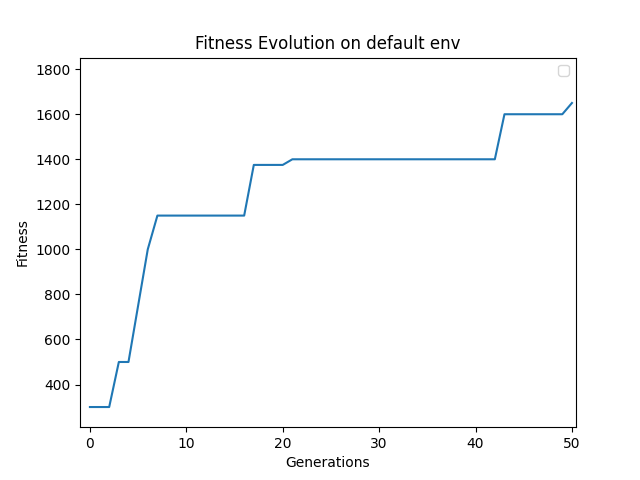
\includegraphics[width=0.5\textwidth]{RapportScientifiqueTemplate/Figure_1.png}
  \caption{Moyenne des fitness des individus sur 50 générations, dans l'env par défaut}
  \label{fig:default}
\end{figure}

\begin{figure}[!htb]
  \centering
  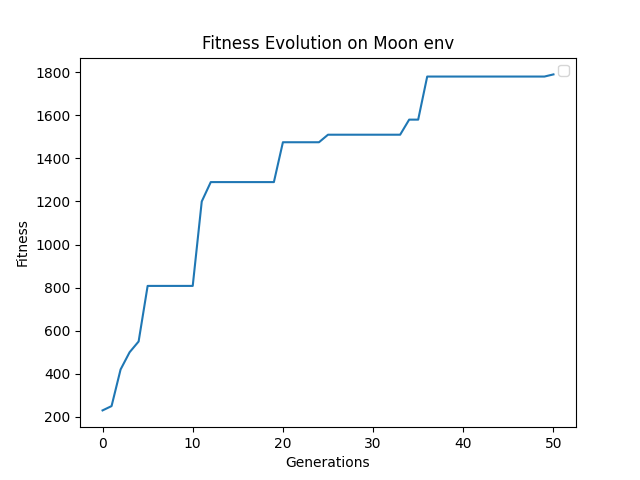
\includegraphics[width=0.5\textwidth]{RapportScientifiqueTemplate/Figure_2.png}
  \caption{Moyenne des fitness des individus sur 50 générations, dans l'env Moon}
  \label{fig:moon}
\end{figure}

Dans ces graphes décrivant les résultats d'un entraînement représentatif, nous pouvons voir que la fitness moyenne des individus augmente au cours des générations. Notons que les résultats d'un entraînement à l'autre peuvent changer de manière significative, mais afficher leur moyenne ne permet pas d'observer efficacement le comportement d'un seul entraînement. 

\begin{figure}[!htb]
  \centering
  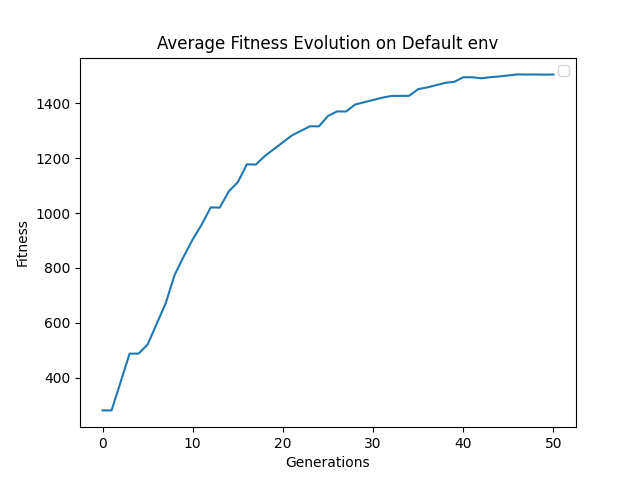
\includegraphics[width=0.5\textwidth]{RapportScientifiqueTemplate/Figure_3.png}
  \caption{Moyenne des entraînements, dans l'env par défaut}
  \label{fig:av}
\end{figure}

Parfois, il peut y avoir des plateaux qui s'étendent sur plusieurs générations. Cela signifie que le génome a atteint un maximum local ou global. L'intérêt de l'étape de mutation est de sortir le génome d'un éventuel maximum local, et c'est ce qu'il semble se passer dans la Figure \ref{fig:default}. A la fin, en revanche, l'algorithme est supposé trouver le maximum global, un plateau est donc attendu. Nous pourrions croire que la Figure \ref{fig:moon} montre ce cas de figure, mais jouer la simulation révélera que la créature ne peut aligner qu'un petit nombre de pas et son progrès est très limité. Cela peut être interpréter de 2 façons différentes. Soit faire tourner l'algorithme pendant une centaine de génération supplémentaires permettra de sortir du maximum local (notons de plus en plus de temps est nécessaire pour sortir des maximums locaux), soit l'état actuel de la fitness function et des autres paramètres de simulation ne permettent pas de trouver d'amélioration au génome et il restera bloqué dans cet état. La seule façon de le savoir serait de faire tourner une série d'entraînements pendant beaucoup plus longtemps, mais nous ne disposons pas des ressources nécessaires pour de tels tests.

\subsection{Discussion}

Durant ce projet, nous avons observé une série de comportements intéressants dû à l'algorithme génétique ainsi que divers problèmes que nous avons dû régler. \\
\\
Premièrement, nous pouvons observer que l'environnement "Moon" donne de meilleurs résultats que l'environnement "Earth" par défaut. Cela est dû aux caractéristiques physiques de ces environnements, en particulier la gravité, plus faible sur Moon. En effet, la gravité plus faible ralenti la chûte de la créature et lui permet de faire de plus grands mouvements avec les mêmes forces qu'elle utiliserait sur Terre.
\\ \\
Concernant la fitness function, nous y avons remarqué un défaut soulignant l'importance de penser à tous les cas de figure. La fitness étant grandement influencée par la vitesse et la distance parcourue, la créature avait tendance à se jeter en avant à la fin du temps imparti de la simulation dans le but de parcourir la plus grande distance. Dans un contexte de robot réel, ce serait un problème qui demanderait de rajouter des conditions complexes à la fitness function pour couvrir ce genre de cas et d'éventuels autres. Dans notre cas, comme cela ne se produit qu'à la fin du temps imparti, c'est peu dérangeant, excepté pour le fait que la créature fini toujours par tomber à la fin. Notons aussi que ce comportement n'est pas présent dans les premières générations et apparaît avec le temps, soulignant l'apprentissage des créatures.

Dans notre fitness function, nous avons aussi essayé plusieurs autres composantes à la formule, que nous avons par la suite choisi de supprimer pour garder (1) comme équation finale.

Une composante abandonnée était la notion de marche droite, qui éviterait que la position $P$ de la créature dévie sur le côté. Ceci est en effet une difficulté supplémentaire de la 3D. Cependant, nous l'avons trouvé trop contraignante en ce qui concerne les mouvements de la créature.

\begin{equation} 
\text{{Walk straight}} = -3 * \text{{ P}}_\text{i-1} * 2
\end{equation}

% Une autre composante qui a été abandonnée car elle ne donnait pas les résultats escomptés était une pénalité qui avait lieu lorsque les joints restaient tournés à leur limite.

Durant notre projet, le principal défi a été l'optimisation.

Dans notre recherche d'optimisation, nous avons aussi cherché à remplacer le génome de forces en génome d'angles. En théorie, contrôler les angles des joints à la place des forces qui leurs sont appliqués permettrait un meilleur contrôle sur les mouvements et leurs limites. Surtout considérant que PyChrono ne présente pas d'unité pour les valeurs des forces, seulement des chiffres difficiles à interpréter quand on ne connaît pas la librairie. Malheureusement, nous n'avons pas identifié d'amélioration significative suite à ce changement de méthode.

Nous avons aussi essayé de changer le génome des forces pour en faire une sorte de matrice discrète. Une valeur sur deux représentant la force à appliquer, l'autre indiquant le temps à attendre avant d'appliquer la force suivante. Nous pensions que ça pourrait considérablement réduire la taille du génome et ainsi grandement améliorer les performances de l'algorithme. Malheureusement, nous nous sommes heurtés à certaines limitations des librairies utilisées, qui nous empêchaient de mettre cette idée en place.






% todo :
% 3D


%	Cette section doit contenir les résultats que vous avez obtenu avec la méthodologie décrite dans la section \ref{sec:met}.
%	Les résultats devront être présentés de préférence sous forme de tableau (cf. Table~\ref{tab:simParameters}) et/ou du diagramme (cf. Fig.~\ref{fig:tf_plot}), et correctement référencés.
%	Les conditions d'expérimentation (c-à-d matériel et logiciels utilisés) devront être ainsi indiquées.
%	En plus des résultats mêmes, cette section devra contenir votre propre analyse et discussion de résultats (par exemple comparaison par rapport à une méthode de référence)

% This is how you define a table: the [!hbt] means that LaTeX is forced (by the !) to place the table exactly here (by h), or if that doesnt work because of a pagebreak or so, it tries to place the table to the bottom of the page (by b) or the top (by t).
%	\begin{table}[!hbt]
		% Center the table
%		\begin{center}
		% Title of the table
%		\caption{Simulation Parameters}
%		\label{tab:simParameters}
		% Table itself: here we have two columns which are centered and have lines to the left, right and in the middle: |c|c|
%		\begin{tabular}{|c|c|}
			% To create a horizontal line, type \hline
%			\hline
			% To end a column type &
			% For a linebreak type \\
%			Information message length & $k=16000$ bit \\
%			\hline
%			Radio segment size & $b=160$ bit \\
%			\hline
%			Rate of component codes & $R_{cc}=1/3$\\
%			\hline
%			Polynomial of component encoders & $[1 , 33/37 , 25/37]_8$\\
%			\hline
%		\end{tabular}
%		\end{center}
%	\end{table}
	
	% This is how you include a eps figure in your document. LaTeX only accepts EPS or TIFF files.
%	\begin{figure}[!hbt]
		% Center the figure.
%		\begin{center}
		% Include the eps file, scale it such that it's width equals the column width. You can also put width=8cm for example...
		%\includegraphics[width=\columnwidth]{plot_tf}
		% Create a subtitle for the figure.
%		\caption{Simulation results on the AWGN channel. Average throughput $k/n$ vs $E_s/N_0$.}
		% Define the label of the figure. It's good to use 'fig:title', so you know that the label belongs to a figure.
%		\label{fig:tf_plot}
%		\end{center}
%	\end{figure}

\section{Conclusion}
%Cette section contient un rappel des contributions / de résultats importants de votre article et éventuellement une indication sur les perspectives de recherche future dans le même domaine.

En conclusion, ce projet nous a permis d'identifier les points clés de la mise en pratique d'un algorithme génétique pour apprendre à une IA à marcher. En particulier l'optimisation du procédé. 

Au début du projet, nous pensions que la principale difficulté serait la mise en place de l'algorithme, la définition de la fitness function et pour aller plus loin, une éventuelle gestion du terrain et c'est pourquoi nous avons choisi de nous aider de PyGad. Contrairement à nos premiers sentiments, l'optimisation était en fait la partie la plus difficile et nous pensons maintenant que coder l'algorithme génétique nous-mêmes aurait rendu le projet plus facile sur le long terme car nous n'aurions pas été limités par une librairie externe.

Une autre optimisation que mettrions en place s'il fallait recommencer le projet serait l'apprentissage en parallèle des tous les individus d'une génération. Le temps pris par entraînement en serait grandement diminué.

% La littérature scientifique nous apprends aussi que 

\bibliographystyle{unsrt}
\bibliography{bibliography}

%\newpage
		
%\appendices
%\section{Consignes}
% Main Part
%\subsection*{Document}
	% LaTeX takes complete care of your document layout ...
%	Le rapport doit être rédigé en \LaTeX{} en utilisant ce template.
%	La longueur du rapport ne devra pas, en tout cas, dépasser les 6 pages.
%	Ce rapport doit être \emph{self-contained}, c-à-d il doit pouvoir être lu et compris sans avoir besoin de se documenter ailleurs.



% Your document ends here!
\end{document}